%!TEX program = xelatex
% Hierarchy charts for the README. Build with ./build.sh, which writes one SVG per diagram.
\documentclass[border=14pt, multi=diagram, varwidth=40cm]{standalone}

\usepackage{fontspec}
\setmainfont{Optima}
\setmonofont{Courier}[Scale=0.88]

\usepackage{xcolor}
\pagecolor{white}
% The same greys as the shaded code blocks in the notes.
\definecolor{shadeA}{RGB}{233,233,233}
\definecolor{shadeB}{RGB}{204,204,204}
\definecolor{rule}{RGB}{90,90,90}

% Labels wrap between words, never inside them.
\hyphenpenalty=10000
\exhyphenpenalty=10000

\usepackage{tikz}
\tikzset{
  handout/.style={line width=0.6pt, draw=rule},
  hbox/.style={draw, line width=0.7pt, rounded corners=2pt, font=\small, align=center,
               minimum height=9mm, inner sep=3pt},
  root/.style={hbox, fill=shadeB, font=\normalsize\bfseries, text width=3.6cm, minimum height=10mm},
  part/.style={hbox, fill=shadeA, font=\small\bfseries, text width=3.6cm},
  leaf/.style={hbox, draw=rule, text width=3.0cm},
}

% \layer{x}{label} draws the top node, centred above the branches.
\newcommand{\layer}[2]{\node[root] (root) at (#1, 0) {#2};}

% \branch{x}{label}{child, child, ...} draws a second-level node hanging from the fork,
% with its children listed underneath it on a rail.
\newcommand{\branch}[3]{%
  \node[part] (part) at (#1, -2) {#2};
  \draw (#1, -1) -- (part.north);
  \foreach \child [count=\i] in {#3}
  {
    \node[leaf, anchor=west] (leaf) at ({#1 - 1.4}, {-2 - 1.2 * \i}) {\child};
    \draw ({#1 - 1.75}, -2.45) |- (leaf.west);
  }
}

% \fork{from}{to} draws the horizontal line joining the root to each branch.
\newcommand{\fork}[2]{\draw (root.south) -- ++(0, -0.55) (#1, -1) -- (#2, -1);}

\newenvironment{diagram}{\centering}{}

\begin{document}

% Kernel
\begin{diagram}
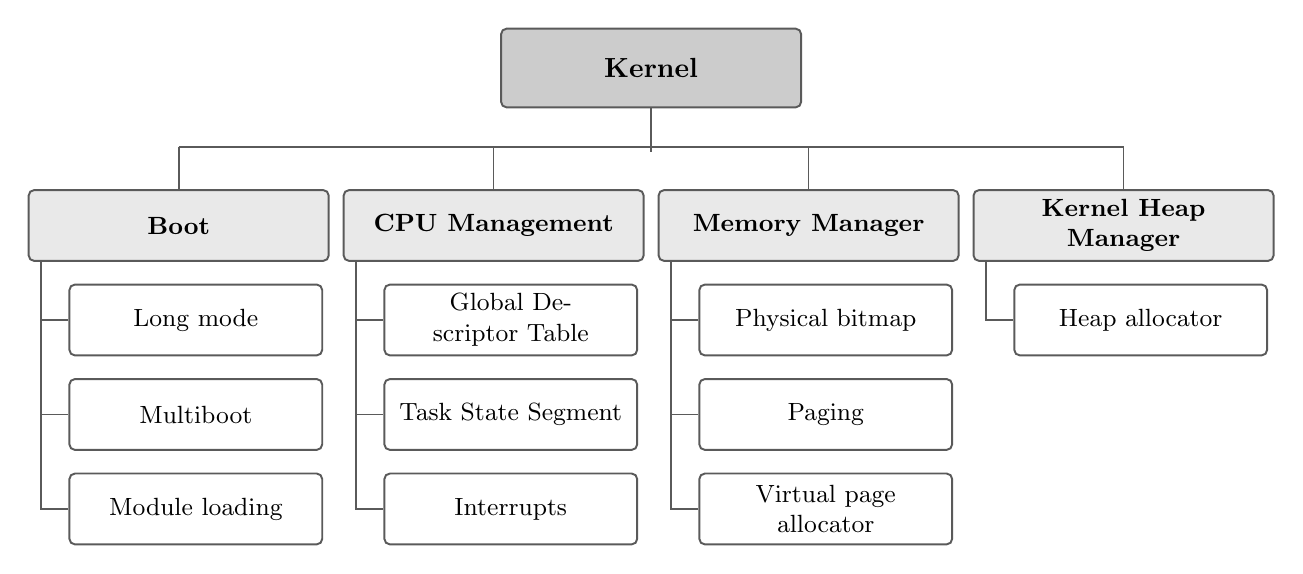
\begin{tikzpicture}[handout]
  \layer{6}{Kernel}
  \fork{0}{12}
  \branch{0}{Boot}{Long mode, Multiboot, Module loading}
  \branch{4}{CPU Management}{Global Descriptor Table, Task State Segment, Interrupts}
  \branch{8}{Memory Manager}{Physical bitmap, Paging, Virtual page allocator}
  \branch{12}{Kernel Heap Manager}{Heap allocator}
\end{tikzpicture}

\vspace{8mm}

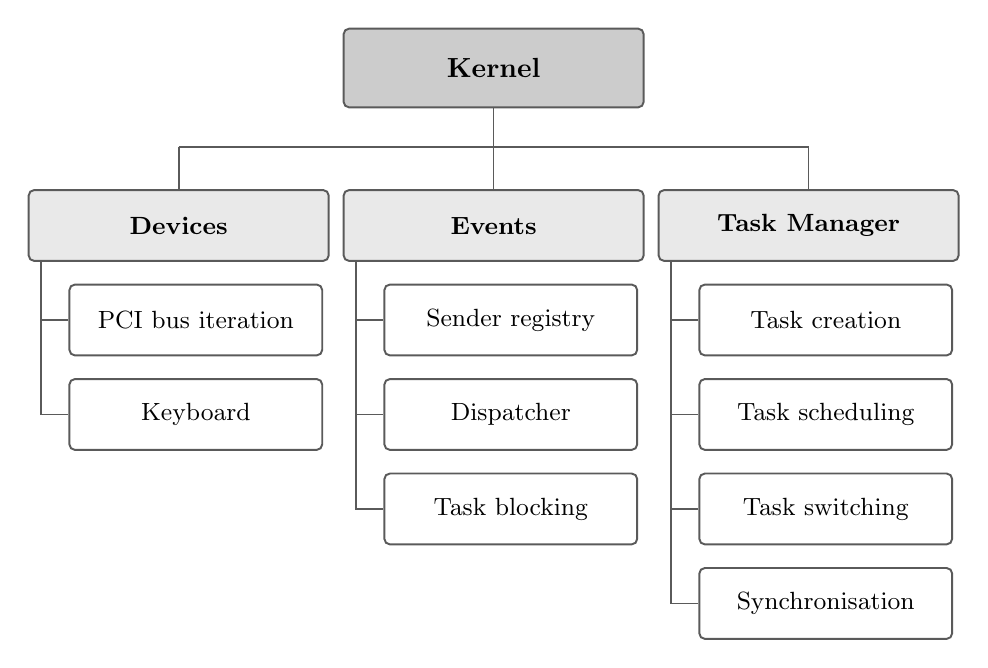
\begin{tikzpicture}[handout]
  \layer{6}{Kernel}
  \fork{2}{10}
  \branch{2}{Devices}{PCI bus iteration, Keyboard}
  \branch{6}{Events}{Sender registry, Dispatcher, Task blocking}
  \branch{10}{Task Manager}{Task creation, Task scheduling, Task switching, Synchronisation}
\end{tikzpicture}
\end{diagram}

% Filesystem layer
\begin{diagram}
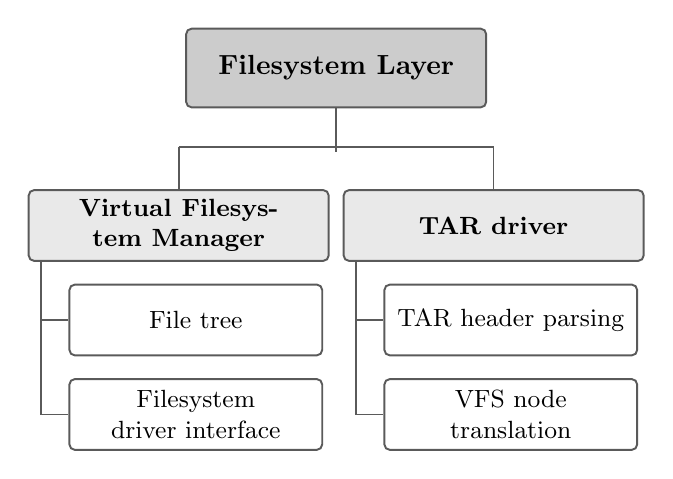
\begin{tikzpicture}[handout]
  \layer{2}{Filesystem Layer}
  \fork{0}{4}
  \branch{0}{Virtual Filesystem Manager}{File tree, Filesystem driver interface}
  \branch{4}{TAR driver}{TAR header parsing, VFS node translation}
\end{tikzpicture}
\end{diagram}

% Networking layer
\begin{diagram}
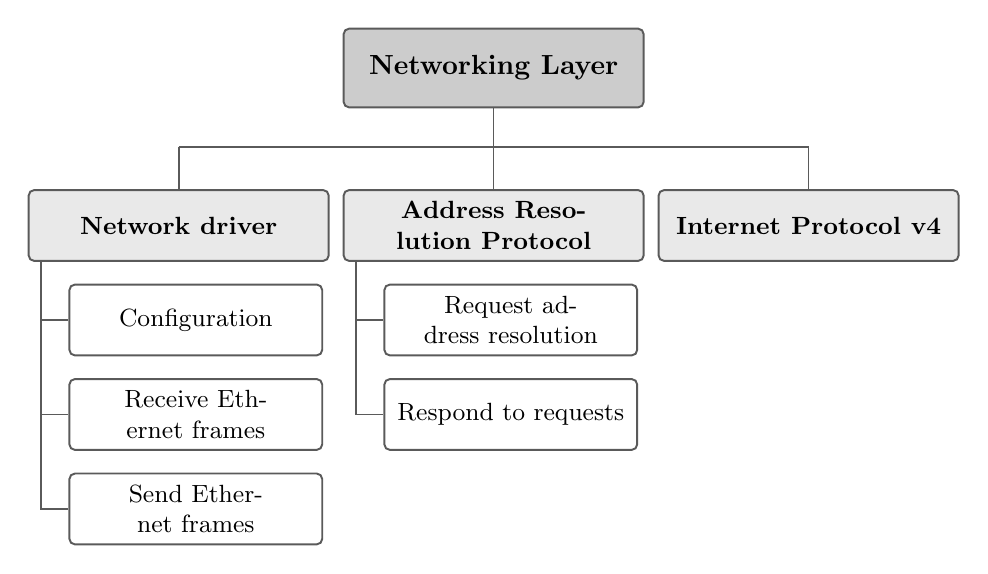
\begin{tikzpicture}[handout]
  \layer{4}{Networking Layer}
  \fork{0}{8}
  \branch{0}{Network driver}{Configuration, Receive Ethernet frames, Send Ethernet frames}
  \branch{4}{Address Resolution Protocol}{Request address resolution, Respond to requests}
  \branch{8}{Internet Protocol v4}{}
\end{tikzpicture}
\end{diagram}

% Internet Protocol v4
\begin{diagram}
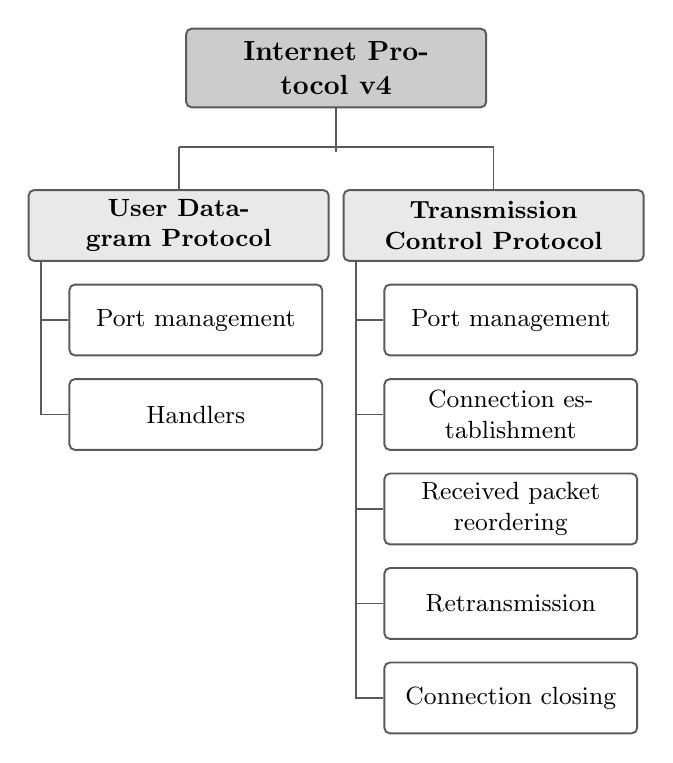
\begin{tikzpicture}[handout]
  \layer{2}{Internet Protocol v4}
  \fork{0}{4}
  \branch{0}{User Datagram Protocol}{Port management, Handlers}
  \branch{4}{Transmission Control Protocol}{Port management, Connection establishment,
    Received packet reordering, Retransmission, Connection closing}
\end{tikzpicture}
\end{diagram}

% User-space
\begin{diagram}
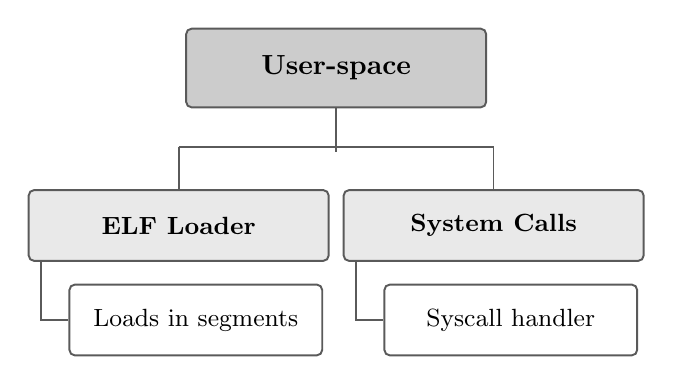
\begin{tikzpicture}[handout]
  \layer{2}{User-space}
  \fork{0}{4}
  \branch{0}{ELF Loader}{Loads in segments}
  \branch{4}{System Calls}{Syscall handler}
\end{tikzpicture}
\end{diagram}

\end{document}
